%Die Angabe des schlauen Spruchs auf diesem Wege funtioniert nur,
%wenn keine Änderung des Kapitels mittels den in preambel/chapterheads.tex
%vorgeschlagenen Möglichkeiten durchgeführt wurde.
%\setchapterpreamble[u]{%
%\dictum[Albert Einstein]{Probleme kann man niemals mit derselben Denkweise lösen, durch die sie entstanden sind.}
%}
\chapter{Implementierung}
\label{chap:impl}
Neben der mathematischen Ausarbeitung (siehe \autoref{chap:maths}) beschäftigt sich diese Arbeit auch mit der eigentlichen Implementierung des erarbeiteten Verfahrens, für welche folgende grundlegenden Anforderungen bestanden:

\begin{description}
\item[Portierbarkeit:] In der Aufgabenstellung war bereits gefordert, dass die Implementierung auf verschiedenen Systemen portierbar sein soll. Aus diesem Grund kamen bereits nur einige wenige Programmiersprachen in Frage.
\item[Evaluation der Daten:] Da die entstehenden Daten auch evaluiert und grafisch dargestellt werden sollten, war eine weitere Anforderung an die Software, dass sie eine \gls{GUI} besitzt oder Bild-Formate exportieren kann.
\item[Funktionalität:] Die Funktionalität der Implementierung stand primär im Vordergrund. An die Performanz der Implementierung und das Design der \gls{GUI} wurden keine besonderen Anforderungen gestellt.
\item[Software-Qualität:] Da diese Arbeit eine Bachelor-Arbeit der Fachrichtung \textit{Softwaretechnik} ist, bestand eine gewisse Anforderung an die Qualität des Quellcodes. Diese beinhaltet u.a. automatisierte Tests, objektorientierte Programmierung und Modulare Strukturen.
\end{description}

Von einer Laufzeitanalyse des Programmes wurde absichtlich abgesehen. Diese Arbeit ist in erster Linie eine Machbarkeitsstudie und erhebt nicht den Anspruch die gestellten Aufgaben in optimaler Zeit zu lösen.

\section{Wahl der Programmiersprache}
\label{sec:language}
Aus den oben beschriebenen Anforderungen ließen sich insgesamt drei mögliche Programmiersprachen ableiten, aus denen eine gewählt werden musste. In die engere Auswahl kamen dabei \texttt{C}, \texttt{C\#} und \texttt{Java}. Aus \autoref{tab:languages} geht hervor, dass alle diese drei Programmiersprachen für den Einsatzzweck dieser Arbeit geeignet wären. Keine der Sprachen erfüllt ein Kriterium gar nicht oder sticht in einem Bereich besonders hervor. Lediglich \texttt{C} verliert durch die wenige Unterstützung von Software-Qualitätsmerkmalen (wie objektorientierte Programmierung, Modularität, Klassen, etc.) an Punkten.

\begin{table}
  \begin{center}
    \begin{tabular}{l|c|c|c|}
	\toprule
      Sprache & \texttt{Java} & \texttt{C} & \texttt{C\#} \\ 
      \midrule
      Portierbarkeit & \checkmark & \checkmark & \checkmark \footnote{Mono (\url{http://www.mono-project.com}) ist eine portierbare Version von C\# die auch auf Unix kompiliert}\\
      \gls{GUI} & \checkmark & \checkmark\footnote{Durch Libraries (z.B. GTK+ \url{http://www.gtk.org}) können in C auch grafische Benutzeroberflächen entwickelt werden } & \checkmark\\
      Objektorientierte Programmierung & \checkmark & $\times$\footnote{Obwohl C keine objektorientierte Sprache ist, ist es grundsätzlich natürlich trotzdem möglich ähnliche Konstrukte zu erzeugen.}  & \checkmark\\
      Automatisierte Tests & \checkmark & \checkmark\footnote{Nicht direkt unterstützt, aber es gibt Testframeworks wie z.B. \url{http://check.sourceforge.net}} & \checkmark\\
      Nativer Systemzugriff\footnote{Der Zugriff auf native Systemfunktionen ermöglicht häufig einen Performance-Gewinn}& $\times$\footnote{Java läuft im sog. \gls{JRE} und hat damit nicht direkt Zugriff auf native Funktionen} & \checkmark & \checkmark\\
	\bottomrule
    \end{tabular}
    \caption{Vergleich der Programmiersprachen \texttt{Java}, \texttt{C} und \texttt{C\#} mit den Anforderungen.}
    \label{tab:languages}
  \end{center}
\end{table}

Aufgrund meiner in universitären Projekte erlangten Vorkenntnissen in \texttt{Java}, wird die Entwicklung der Software für diese Arbeit in derselbigen Sprache geschehen.

Für die grafische Evaluation der Ergebnisse wurde in der vorliegende Arbeit eine \texttt{SWING}-Oberfläche, die sowohl die Eingabe der Parameter und Daten sowie die Ausgabe der verschiedenen Diagramme und Bilder ermöglichen soll.

Die \autoref{fig:tool} zeigt die einfach gehaltene Oberfläche mit den möglichen Einstellungen.

\section{Externe Bibliotheken}
Für die Implementierung wurden einige bereits bestehenden Komponenten eingesetzt. Diese werden hier kurz beschrieben.

\subsubsection*{\texttt{NumericTextField}\footnote{\url{http://www.java2s.com/Code/Java/Swing-JFC/NumericTextField.htm}}}
Für die Eingabe der einzelnen Parameter wird eine Implementierung eines numerischen Textfeldes verwendet. Dieses verhindert ungültige Eingaben und erleichtert das Auslesen der numerischen Parameter.

\subsubsection*{\texttt{metadata-extractor}\footnote{\url{https://code.google.com/p/metadata-extractor/}}}
Die Bibliothek \texttt{metadata-extractor} wird verwendet um automatisiert aus Bilddateien die Belichtungszeit der Bilder auszulesen. Mit dieser wird auch das von Adobe entwickelte \texttt{xmp-core}\footnote{\url{http://www.adobe.com/devnet/xmp.html}} mit geliefert. Zusammen ermöglichen es die Bibliotheken die Belichtungszeiten der Bilder auszulesen und darzustellen.

\subsubsection*{\texttt{JImageChooser} \footnote{\url{http://docs.oracle.com/javase/tutorial/uiswing/examples/components/index.html\#FileChooserDemo2}}} 
Der verwendete \texttt{JFileChooser} zur Selektion der Bilddateien ist inspiriert von dem vorhandenen Tutorial bei Oracle. Er ist in der Lage eine kleine Vorschau der Bilder anzuzeigen.


\section{Architektur}
\label{sec:architektur}
Bei der Architektur der Software wurde eine \gls{MVC} Struktur eingehalten. Dieses Pattern beschreibt eine klare Trennung zwischen Datendarstellung, -verarbeitung und -repräsentation. Diese Teilung in drei Schichten sorgt dafür, dass die einzelnen Komponenten gut getestet werden können und beliebig austauschbar sind. Dadurch besteht ein hoher Grad an Erweiterbarkeit, da die Kopplung zwischen den Modulen möglichst gering gehalten wird \cite[S.~413]{ludewig}.

In allen Klassen wurde grundsätzlich das Prinzip des Information Hiding angewandt. Dadurch kann die innere Arbeit der Klassen und Module möglichst unabhängig ablaufen, was eine Erweiterbarkeit vereinfacht.



\begin{ieee}{information hiding}
A software development technique in which each module's interfaces reveal a s little a s possible about the module's inner workings and other modules are prevented from using information about the module that is not in the module's interface specification.
\end{ieee}

\subsection{Komponentendiagramm}
Die Anwendung lässt sich grundsätzlich in fünf verschiedene Komponenten trennen (siehe \autoref{fig:arch:components}). 
\begin{description}

\item{\texttt{View}:} Das Paket \texttt{View} behandelt die gesamte Darstellung der Anwendung und die grafische Auswertung der berechneten Bilder. Es enthält \gls{Tone-Mapping}-Operatoren und behandelt die Benutzereingabe.

\item{\texttt{Model}:} Das \texttt{Model} besteht in erster Linie aus den beiden Klassen \texttt{Image} und \texttt{HDRResult} und ist damit ein Datentypmodul \cite[S. 412]{ludewig}. Erstere wird als Repräsentation eines Bildes verwendet und speichert Grauwerte, Belichtungszeiten und weitere bildrelevante Informationen. Letztere dient als Kommunikationspaket zwischen dem eigentlichen \texttt{Solver} und der restlichen Anwendung und enthält die fertig berechnete Antwortkurve und die \gls{Radiance Map}.

\item{\texttt{Solver}:} Der \texttt{Solver} ist der eigentliche Kern des Programms. In diesem Paket wird die Bestimmung der Antwortkurve $\b g$ sowie die Berechnung der \gls{Radiance Map} behandelt. Hier fließen die mathematischen Erkenntnisse aus \autoref{chap:maths} ein.

\item{\texttt{Ctrl}:} Dieses Paket dient zur Steuerung der Anwendung. In diesem werden die Eingaben verarbeitet, an die Algorithmen übergeben und anschließend wieder dargestellt.

\item{\texttt{Maths}:} Die \texttt{Maths}-Komponente ist ein Funktionales Modul \cite[S. 412]{ludewig}. Es enthält alle notwendigen mathematischen Berechnungen und Repräsentationen, wie z.B. \texttt{Matrix} und \texttt{Vector}.
\end{description}


Nachfolgend wird nun auf die einzelnen Komponenten und Klassen näher eingegangen (siehe \autoref{fig:arch:view}). Die \texttt{View} besteht in erster Linie aus der Klasse \texttt{GuiFrame}. Diese ist das eigentliche Fenster des Programms und übernimmt die Schnittstelle zwischen Anwender und Programm. 

Darin enthalten sind auch die verschiedenen \texttt{ToneMappers}, die zur Darstellung der \gls{Radiance Map} verwendet werden. Zusammen mit dem Paket \texttt{Plots} wird eine detailliertere Ansicht auf die beteiligten Klassen in \autoref{fig:arch:plots} dargestellt.

\begin{figure}[H]
  \begin{center}
    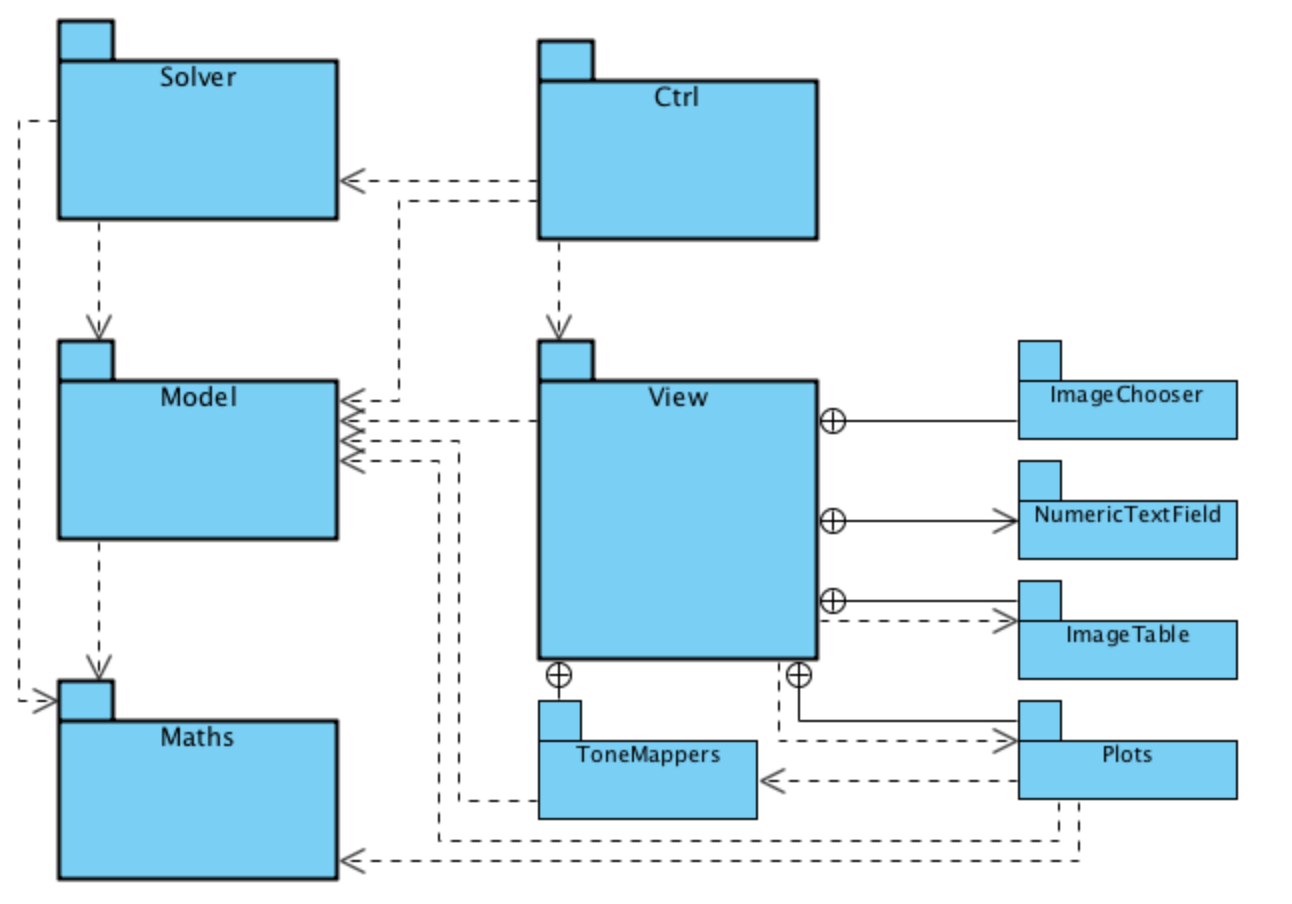
\includegraphics[width=0.6\textwidth]{architecture/components}
    \caption{Die Architektur der Software auf Komponentenebene. Die Trennung zwischen den einzelnen Bereichen ist hier deutlich erkennbar.}
    \label{fig:arch:components}
  \end{center}
\end{figure}


\begin{figure}[H]
  \begin{center}
    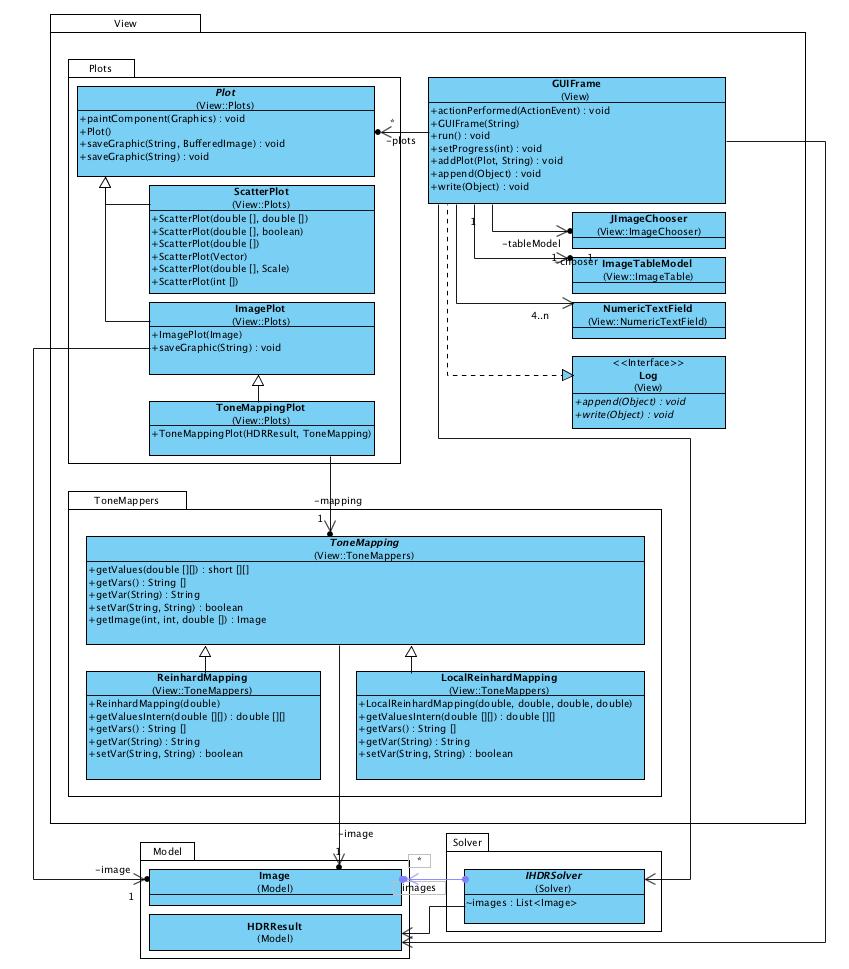
\includegraphics[width=0.9\textwidth]{architecture/view}
    \caption{Die \texttt{View}-Komponente im Detail. Das Hauptfenster \texttt{GUIFrame} stellt die Daten dar und importiert dazu die verschiedenen Komponenten. Die \texttt{Plots} und die \texttt{ToneMappers} gehören ebenfalls zu diesem Paket.}
    \label{fig:arch:view}
  \end{center}
\end{figure}


\begin{figure}[H]
  \begin{center}
    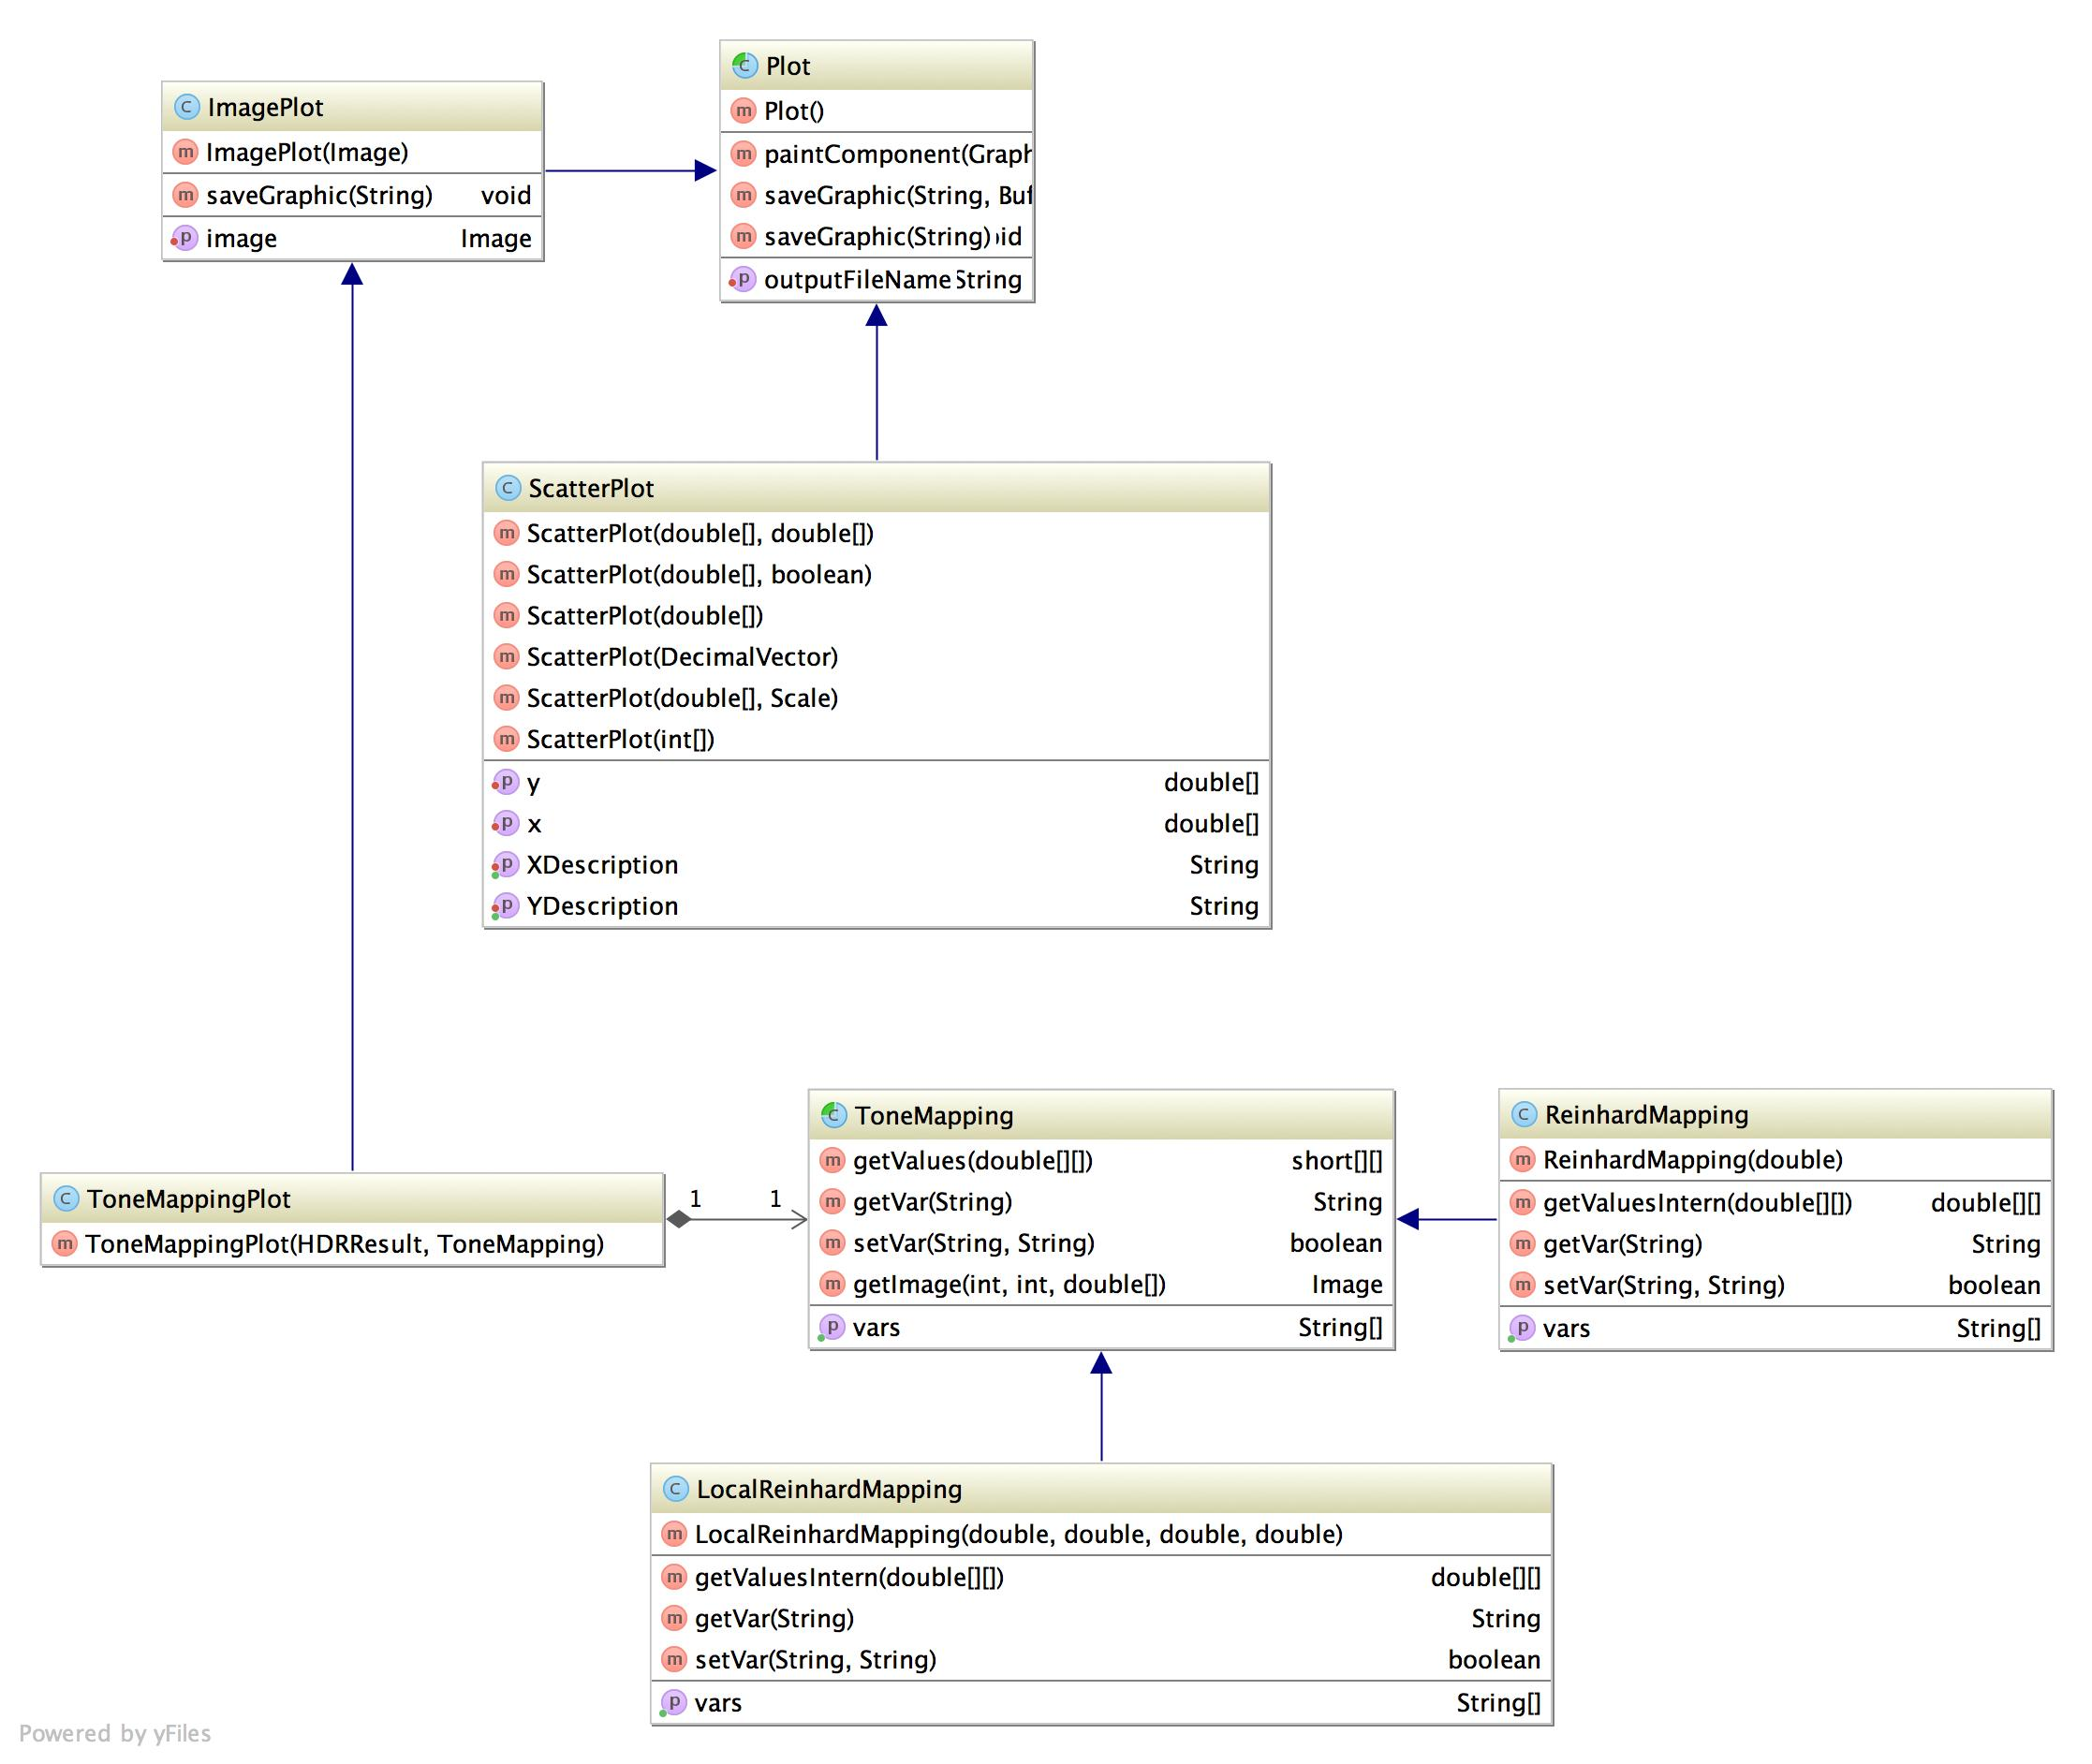
\includegraphics[width=\textwidth]{architecture/plots}
    \caption{Die Struktur der verschiedenen grafischen Plots. Die verschiedenen \gls{Tone-Mapping}-Operatoren wurden mittels Vererbung implementiert.}
    \label{fig:arch:plots}
  \end{center}
\end{figure}

Einige der mathematischen Aufgaben (wie z.B. die LU-Zerlegung oder das SOR-Verfahren, siehe \autoref{sec:solvers}) sind im Paket \texttt{Maths} ausgelagert. Die abstrakte Klasse \textit{Matrix} stellt die Basisfunktionalität zur Verfügung und kennt die beiden Implementierungen \texttt{BandMatrix} und \texttt{DefaultMatrix}. Erstere ist eine spezielle Repräsentation von dünnbesetzten Diagonalmatrixen mit beliebig vielen Bändern. Die hier häufig beschriebenen pentadiagonal Matrizen werden mit dieser Implementierung dargestellt. Der Vorteil dieser ist, dass auch große sehr dünn besetzte Matrizen abgespeichert werden können (in einem zweidimensionalen Array würden diese zu viel Speicherplatz verbrauchen). Die \texttt{DefaultMatrix} ist die zweite Implementierung der Matrizen und arbeitet intern mit einem zweidimensionalen Array.

\begin{figure}[H]
  \begin{center}
    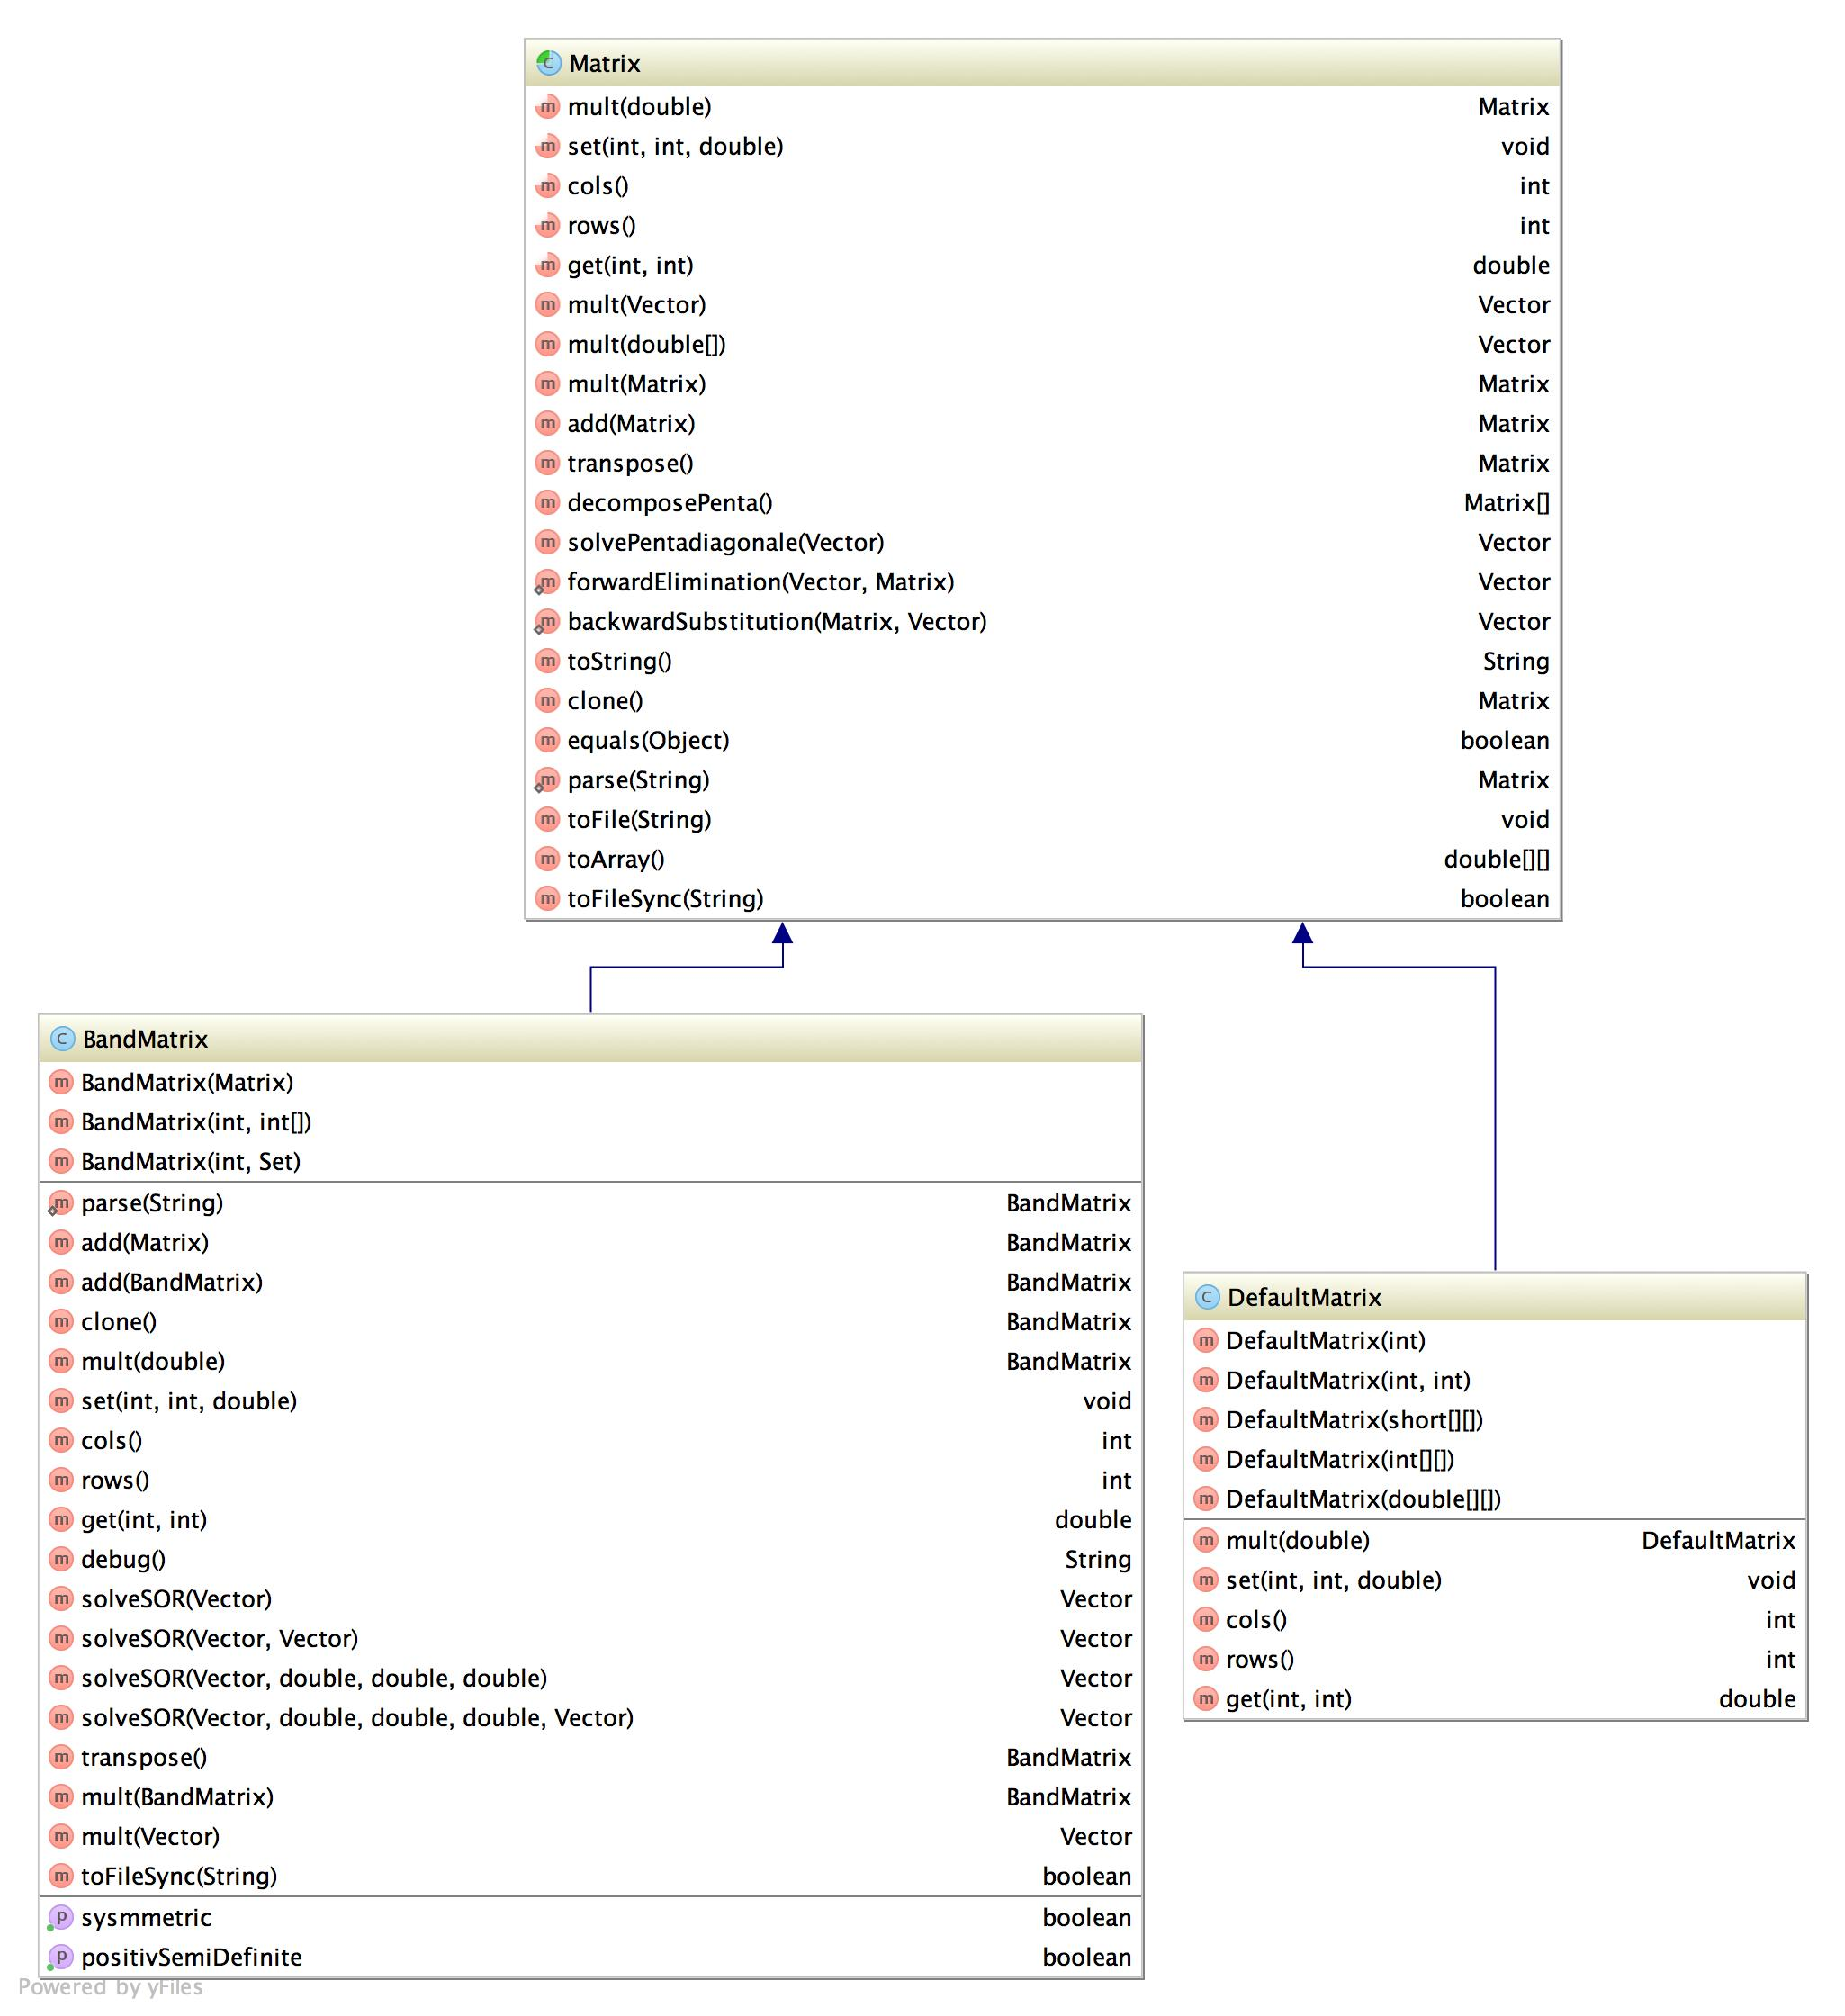
\includegraphics[width=\textwidth]{architecture/matrixes}
    \caption{Die Klasse \texttt{Matrix} und ihre Spezialisierungen \texttt{BandMatrix} und \texttt{DefaultMatrix}. Diese beiden Klassen dienen zusammen mit \texttt{Vector} als ein Kernbestandteil der mathematischen Berechnungen dieses Programms.}
    \label{fig:arch:matrix}
  \end{center}
\end{figure}


\begin{figure}[H]
  \begin{center}
    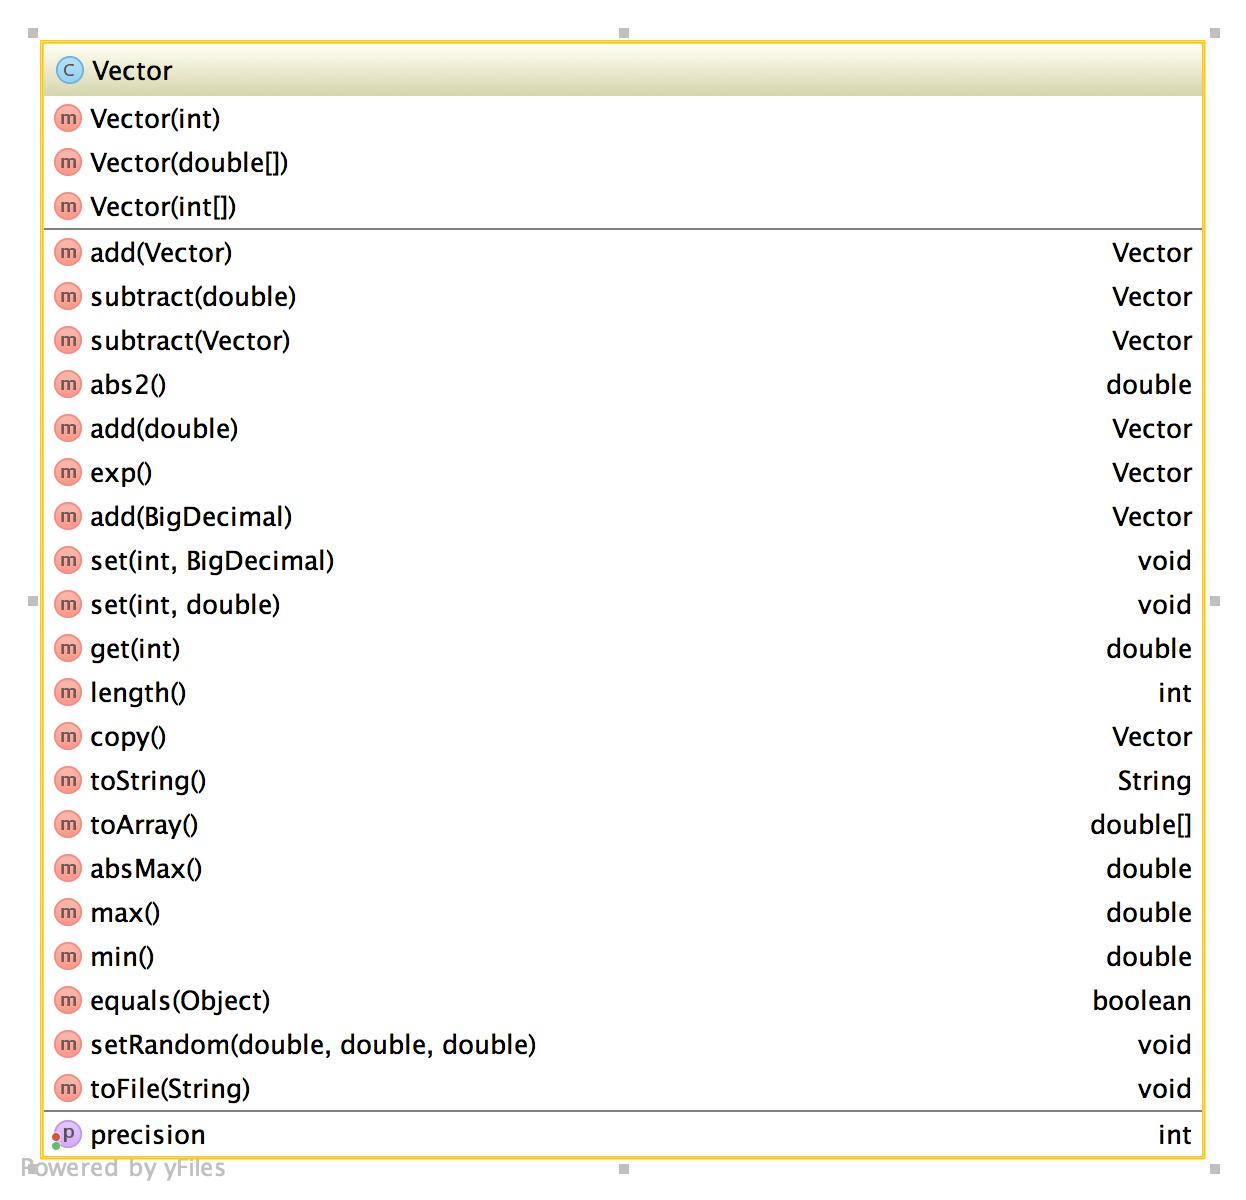
\includegraphics[width=9cm]{architecture/vector}
    \caption{Die Klasse \texttt{Vector} dient zur Kapselung von Funktionen mit Vektoren und Matrizen.}
    \label{fig:arch:vector}
  \end{center}
\end{figure}


\subsection{Sequenzdiagramm}
Das Programm läuft sehr vielschichtig ab. Als grundsätzlicher Informationsfluss dient der Aufbau wie er in \autoref{fig:arch:sequence} beschrieben. Wichtig dabei ist, dass die grafische Benutzeroberfläche nicht von der Berechnungsdauer des Algorithmus blockiert wird, weshalb besonders zwischen \texttt{Controller} und \texttt{GUIFrame} asynchrone Methodenaufrufe eingesetzt werden.
\begin{figure}[H]
  \begin{center}
    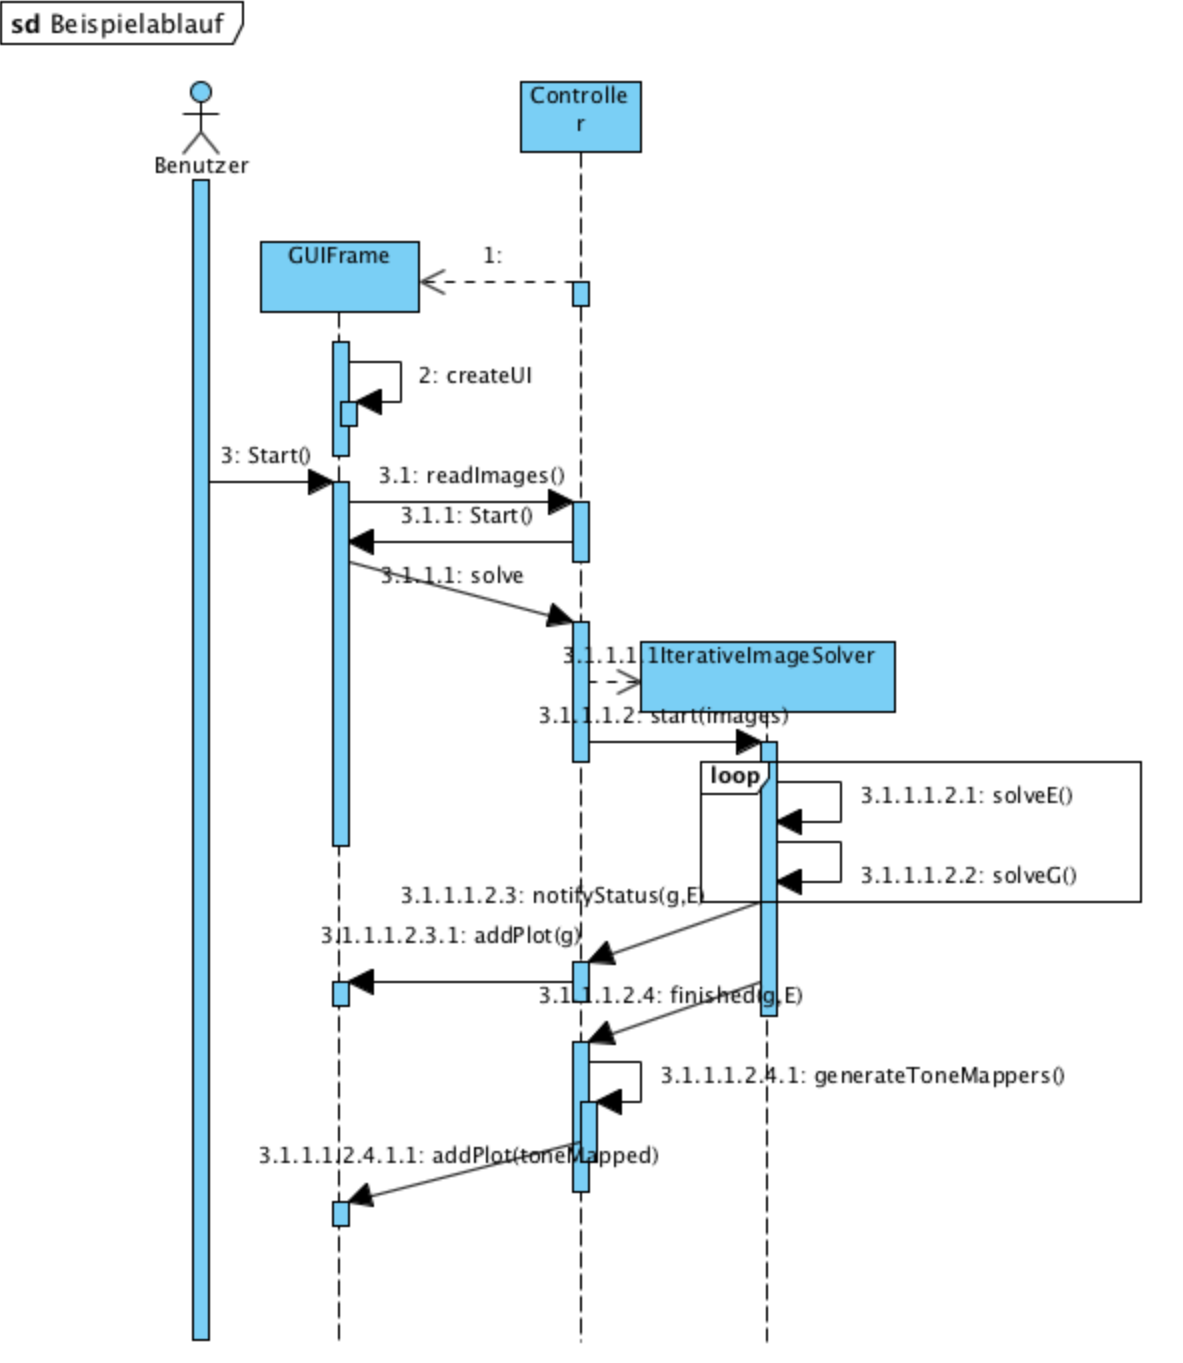
\includegraphics[width=0.8\textwidth]{architecture/sequence_example}
    \caption{Der grundsätzliche Ablauf der Berechnung des HDR-Bildes und der Antwortkurve und der dabei beteiligten Komponenten sowie deren Interaktion. }
    \label{fig:arch:sequence}
  \end{center}
\end{figure}

\section{Programmvorstellung}
\label{sec:sample-codes}
Die gesamte implementierte Anwendung befindet sich auf der beigefügten CD-Rom zu dieser Arbeit oder kann unter \url{https://github.com/sebastianzillessen/hdr-generator} heruntergeladen werden. Das \texttt{JAR}-Archiv kann dann einfach ausgeführt werden.

\begin{figure}
  \begin{center}
    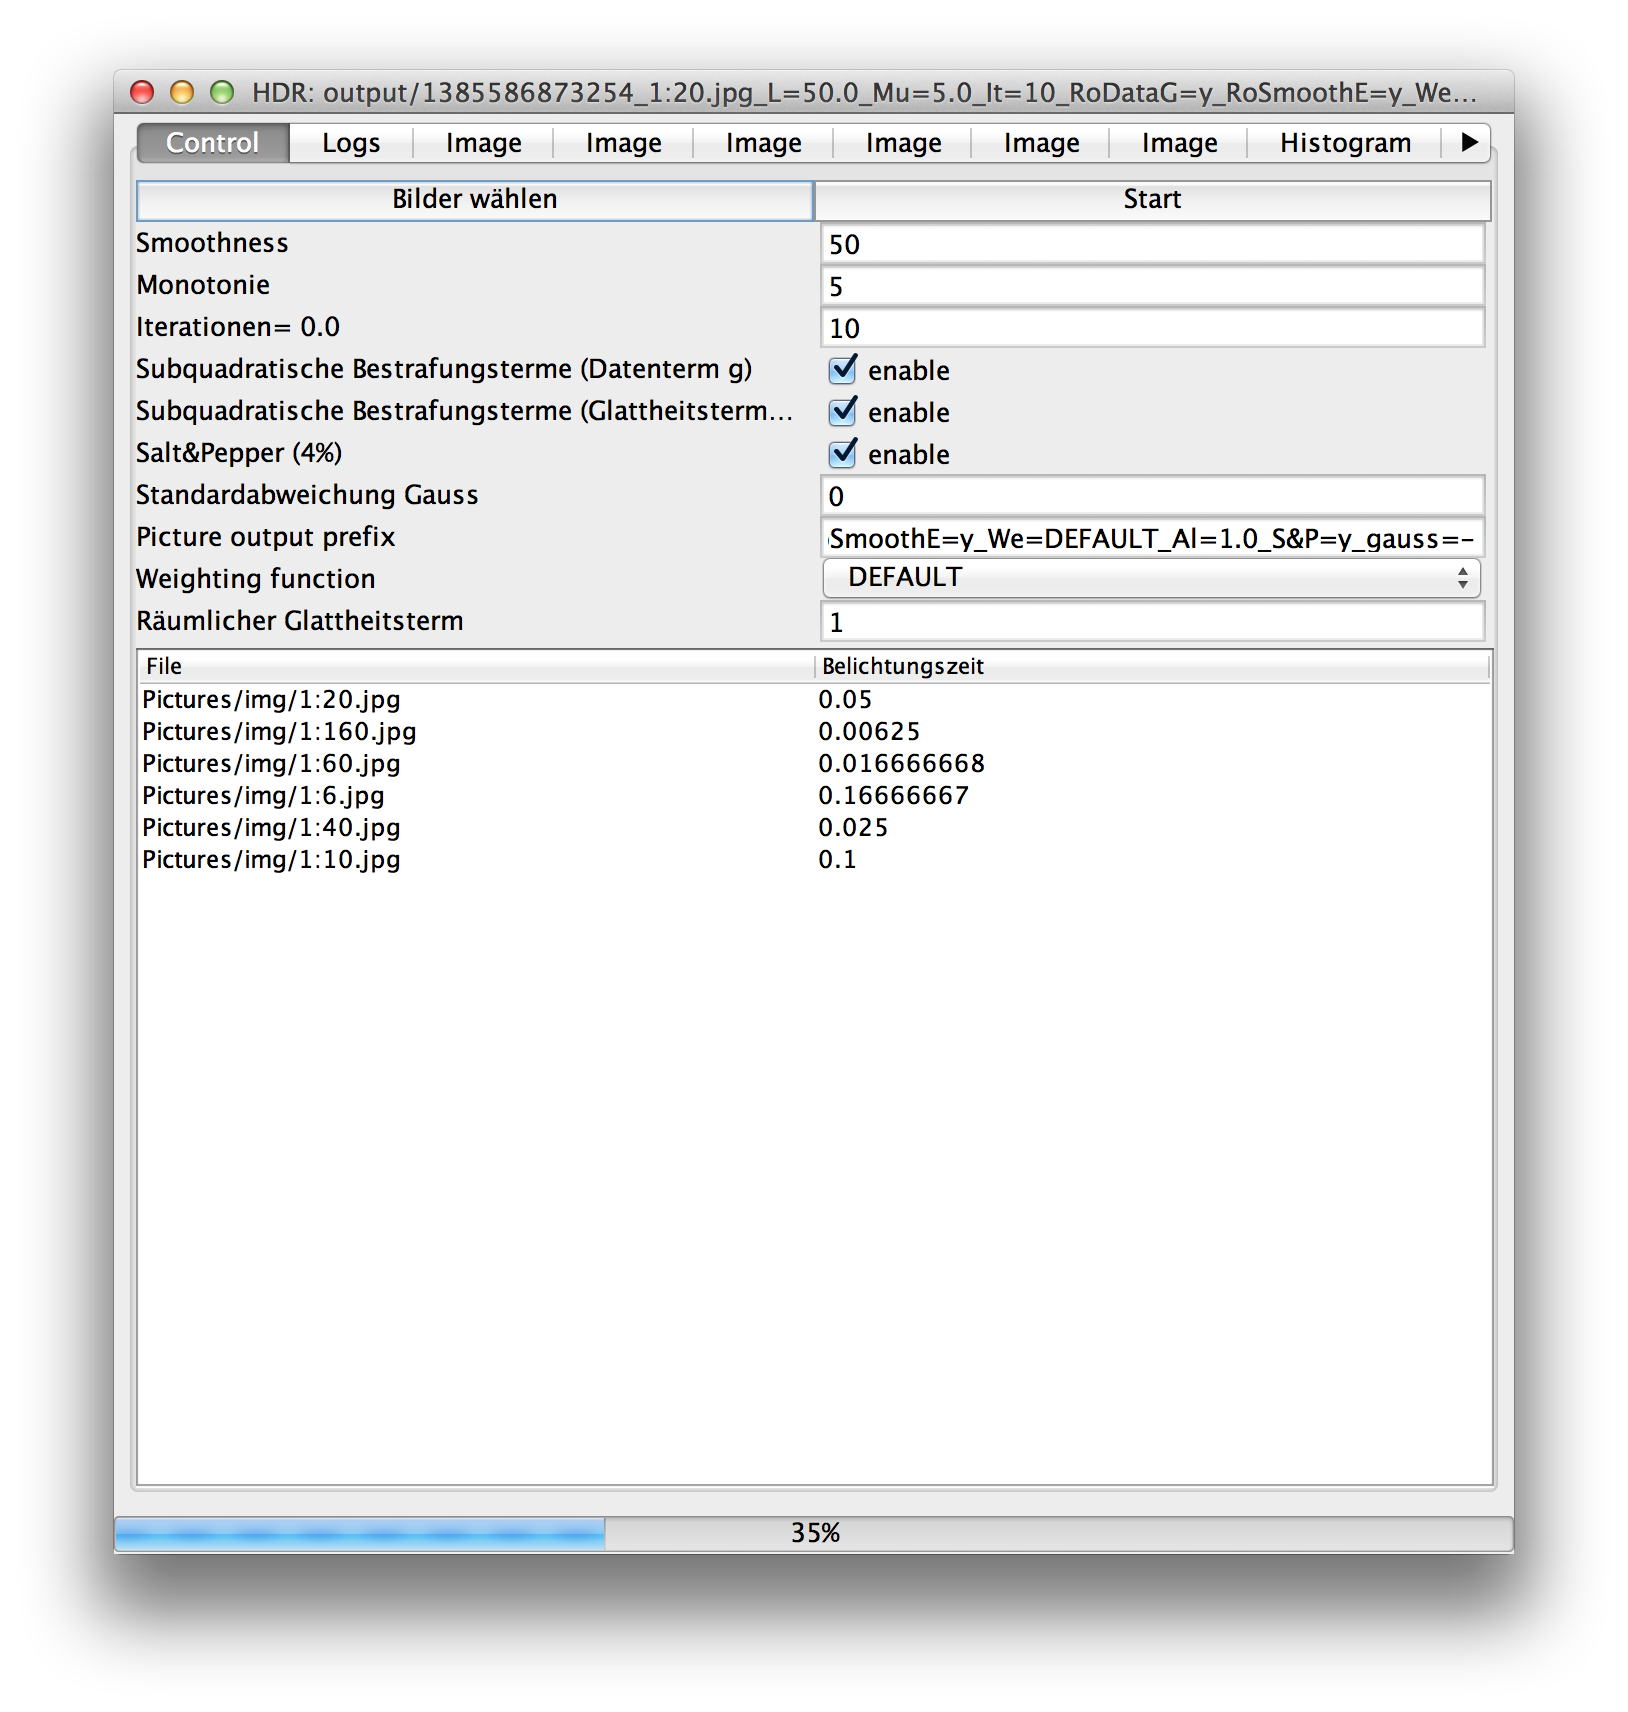
\includegraphics[width=\textwidth]{Tool}
    \caption{Die Benutzereingabe für die Erzeugung der HDR-Bilder ist absichtlich schlicht und einfach gehalten.}
    \label{fig:tool}
  \end{center}
\end{figure}

Die Software unterstützt bisher keine Registrierung der Bilder. D.h. die Bilder müssen vorab von Hand oder mit einem Algorithmus registriert werden und können dann mit diesem Programm verwendet werden.

Zunächst müssen über den Button \enquote{Bilder wählen} die Eingabebilder gewählt werden (siehe \autoref{fig:images}). Sobald die Bilder geladen wurden, erscheinen diese in der unteren Auflistung. Die Belichtungszeit wird in der Tabelle mit angegeben, falls durch die Bibliothek \texttt{metadate-extractor} diese Information bereits ausgelesen wurde. Ansonsten müssen diese händisch eingegeben werden.

Die Eingabemöglichkeiten im oberen Bereich des Fensters dienen der Parametrisierung  der Anwendung. Hier können insbesondere die Einstellungen zur Monotonie-Forderung, dem räumlichen Glattheitsterm oder den robusten Bestrafungsfunktionen vorgenommen werden.

\begin{figure}
  \begin{center}
    \includegraphics[width=0.6\textwidth]{images}
    \caption{Auswahl der Belichtungsserie incl. Vorschau.}
    \label{fig:images}
  \end{center}
\end{figure}

Außerdem können zu Testzwecken Bildstörungen (\gls{SaltAndPepperNoise} oder additives Gauss-Rauschen) aktiviert werden, wodurch die verschiedenen Verfahren verglichen werden können. Die Ausgabe (auch der Zwischenresultate) erfolgt über die verschiedenen Reiter des Fensters. Darüber hinaus werden die Resultate (globaler und lokaler Reinhard \gls{Tone-Mapping}-Operator) in diesen ausgegeben (siehe \autoref{fig:app:tone}). Der Fortschritt des Verfahrens wird im unteren Bereich der Anwendung dargestellt.

Jeder der verschiedenen Graphen oder Plots kann gespeichert werden. Dazu steht ein Speichern-Button zur Verfügung. 
Der Funktionsumfang der Anwendung wurde absichtlich schmal gehalten, da der Fokus auf der Erweiterung des Ansatzes und nicht auf der Erstellung einer High-End-Software lag.

\begin{figure}
  \begin{center}
    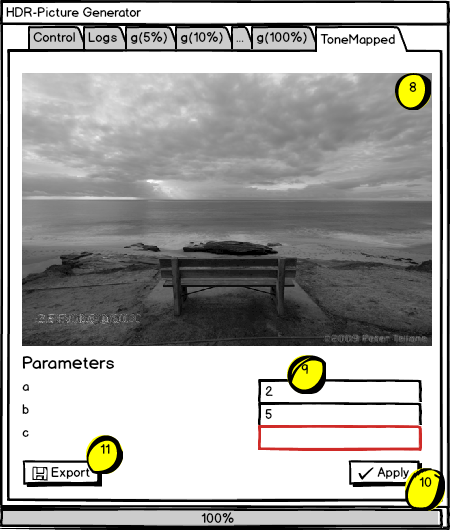
\includegraphics[width=0.6\textwidth]{tonemapped}
    \caption{Vorschau des Tone-Mapped Resultats mit der Möglichkeit der Veränderung der Variablen für diesen Tone-Mapper (globaler \gls{Tone-Mapping}-Operator von Reinhard).}
    \label{fig:app:tone}
  \end{center}
\end{figure}


\section{Herausforderungen während der Programmierung}